\phantomsection
\subsection{(10\%) Sử dụng phần mềm VirtualBox/VMware/UTM/Parallels}

\begin{itemize}
  \item[--] Tạo 1 Nat Network tên "QTHT" có địa chỉ mạng là 10.0.2.0/24. Tắt dịch vụ DHCP có sẵn trên NAT Network "QTHT".
  \item[--] Tạo 2 máy ảo với thông tin như sau: \\
    \begin{minipage}{\linewidth}
      \begin{multicols}{2}
        \begin{minipage}{\linewidth}
          \captionsetup{type=table}
          \caption{\bfseries Cấu hình máy Server}
          \centering
          \begin{tabular}{| m{.46\linewidth} | m{.42\linewidth} |}
            \hline
            \textbf{Hostname}                                       & Server                                                               \\\hline
            \parbox[c][2.5cm][c]{\linewidth}{\textbf{Hệ điều hành}} & \parbox[c][2.5cm][c]{\linewidth}{CentOS 9}                           \\\hline
            \textbf{CPU / RAM / DISK}                               & 1core/2G/10G \newline Hoặc tùy chỉnh theo cấu hình máy của sinh viên \\\hline
            \textbf{Network}                                        & NAT Network \newline Name: "QTHT"                                    \\\hline
            \textbf{IP}                                             & 10.0.2.2                                                             \\\hline
            \textbf{Subnet mask}                                    & 255.255.255.0                                                        \\\hline
            \textbf{Gateway}                                        & 10.0.2.1                                                             \\\hline
            \textbf{DNS}                                            & 10.0.2.1                                                             \\\hline
          \end{tabular}
        \end{minipage}

        \begin{minipage}{\linewidth}
          \captionsetup{type=table}
          \caption{\bfseries Cấu hình máy Desktop}
          \centering
          \begin{tabular}{| m{.46\linewidth} | m{.42\linewidth} |}
            \hline
            \textbf{Hostname}                                                                                 & Desktop                                                                                 \\\hline
            \parbox[c][2.5cm][c]{\linewidth}{\textbf{Hệ điều hành}}                                           & \parbox[c][2.5cm][c]{\linewidth}{Lubuntu 22.04, \newline hoặc bất kỳ hệ điều hành khác} \\\hline
            \textbf{CPU / RAM / DISK}                                                                         & 1core/2G/20G \newline Hoặc tùy chỉnh theo cấu hình máy của sinh viên                    \\\hline
            \textbf{Network}                                                                                  & NAT Network \newline Name: "QTHT"                                                       \\\hline
            \parbox[c][2.69cm][c]{\linewidth}{\textbf{IP \newline Subnet mask \newline Gateway \newline DNS}} & \parbox[c][2.69cm][c]{\linewidth}{Cấu hình tự động sử dụng dịch vụ DHCP}                \\\hline
          \end{tabular}
        \end{minipage}
      \end{multicols}
    \end{minipage}

    \vspace{.3cm}
    \textbf{Lưu ý:}
    \begin{itemize}
      \item[+] Trong quá trình cài hệ điều hành CentOS 9, tạo 1 tài khoản với username là mã số sinh viên; firstname và lastname là họ tên của sinh viên. Cấp quyền quản trị (sudo) cho tài khoản. Sử dụng tài khoản vừa tạo để thực hiện bài tập tổng hợp (không dùng tài khoản root).
    \end{itemize}
\end{itemize}

% =========================================================
\phantomsection
\subsubsection{Tạo 1 NAT Network tên "QTHT"}

\begin{minipage}{.93\linewidth}
  \captionsetup{type=figure, skip=-15pt}
  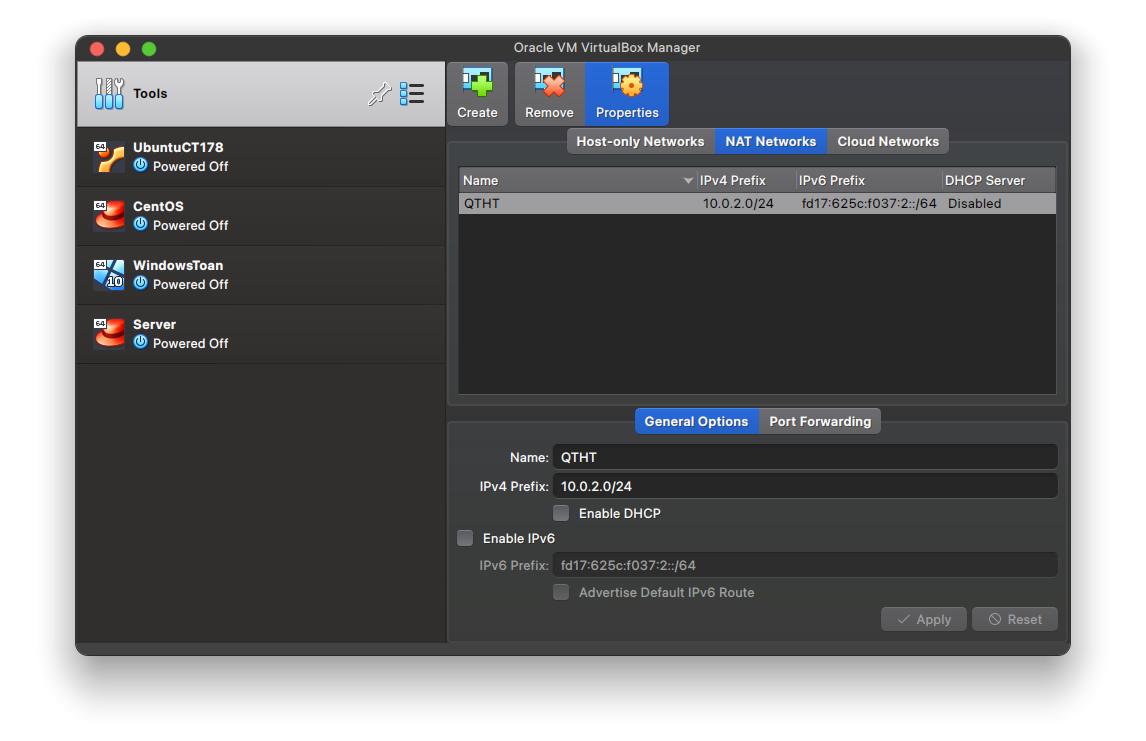
\includegraphics[width=\linewidth]{./imgs/Hinh-2.png}
  \caption{\bfseries Cấu hình NAT Network QTHT}
\end{minipage}

% =========================================================
\phantomsection
\subsubsection{Tạo 2 máy ảo Server và Desktop}

\paragraph{Server có cấu hình như sau:}

\begin{itemize}
  \item Hệ điều hành: CentOS 9
  \item CPU: 1 Core \textit{(\myref{fig:server-processor})}
  \item Ram: 4GB \textit{(\myref{fig:server-ram})}
  \item Disk: 10GB \textit{(\myref{fig:server-disk})}
  \item Network: NAT Network "QTHT" \textit{(\myref{fig:server-network-1})}
  \item IPv4: 10.0.2.2 \textit{(\myref{fig:server-network-2})}
  \item Subnet mask: 255.255.255.0 \textit{(\myref{fig:server-network-2})}
  \item Gateway: 10.0.2.1 \textit{(\myref{fig:server-network-2})}
  \item DNS: 10.0.2.1 \textit{(\myref{fig:server-network-2})}
\end{itemize}





\begin{minipage}{.93\linewidth}
  \captionsetup{type=figure, skip=-15pt}
  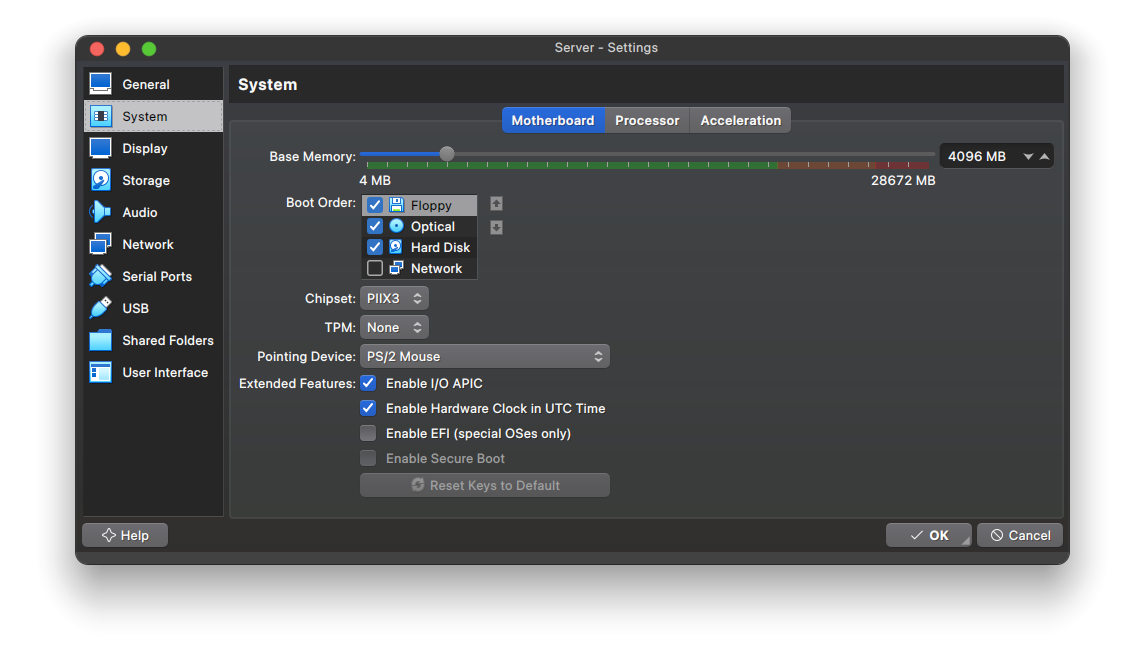
\includegraphics[width=\linewidth]{./imgs/Hinh-3.png}
  \caption{\bfseries Dung lượng Ram của Server}
  \label{fig:server-ram}
\end{minipage}


\begin{minipage}{.93\linewidth}
  \captionsetup{type=figure, skip=-15pt}
  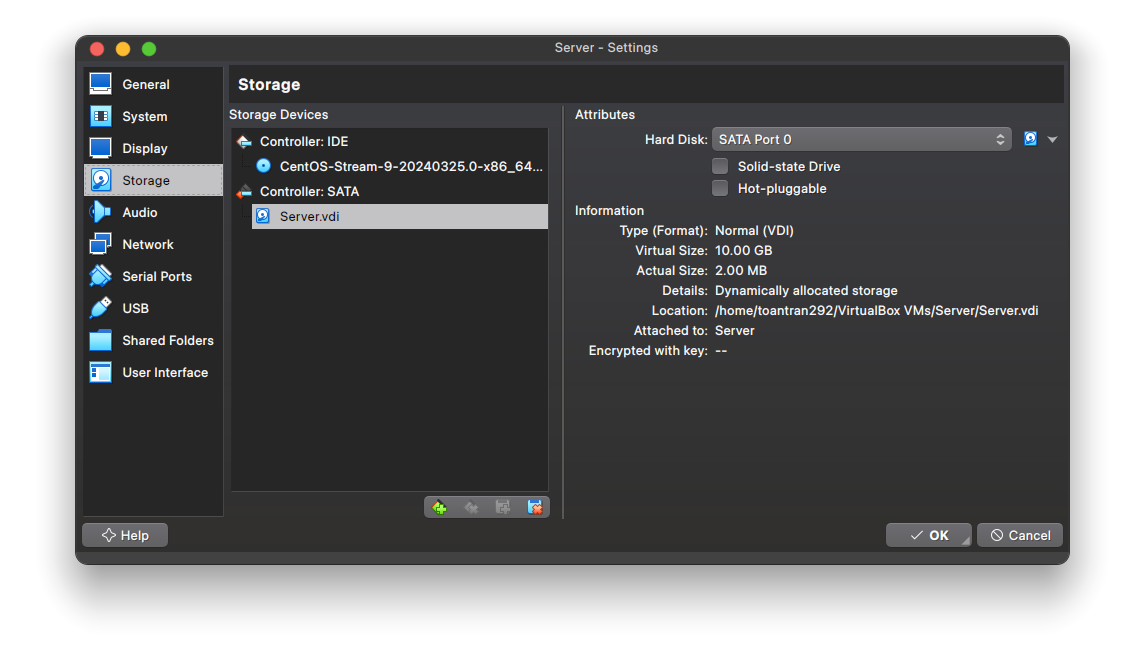
\includegraphics[width=\linewidth]{./imgs/Hinh-5.png}
  \caption{\bfseries Dung lượng ổ cứng của Server}
  \label{fig:server-disk}
\end{minipage}


\begin{minipage}{.93\linewidth}
  \captionsetup{type=figure, skip=-15pt}
  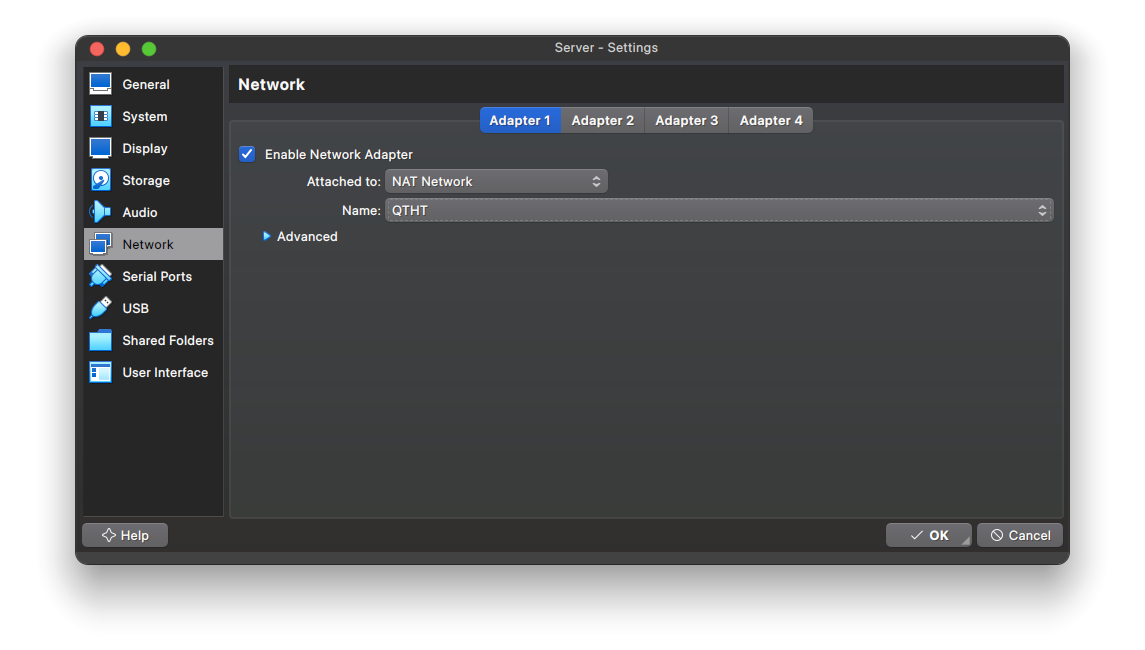
\includegraphics[width=\linewidth]{./imgs/Hinh-6.png}
  \caption{\bfseries Cấu hình mạng máy tính Server}
  \label{fig:server-network-1}
\end{minipage}


\begin{minipage}{.93\linewidth}
  \captionsetup{type=figure}
  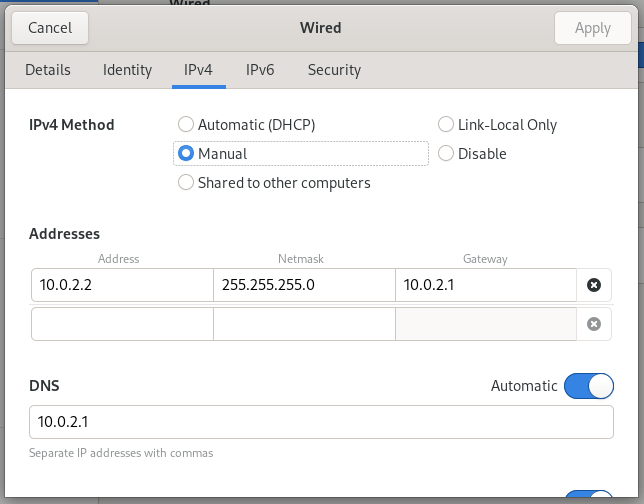
\includegraphics[width=\linewidth]{./imgs/Hinh-7.png}
  \caption{\bfseries Cấu hình mạng máy tính Server}
  \label{fig:server-network-2}
\end{minipage}


\paragraph{Desktop có cấu hình như sau:}

\begin{itemize}
  \item Hệ điều hành: CentOS 9
  \item CPU: 1 Core \textit{(\myref{fig:desktop-processor})}
  \item Ram: 4GB \textit{(\myref{fig:desktop-ram})}
  \item Disk: 20GB \textit{(\myref{fig:desktop-disk})}
  \item Network: NAT Network "QTHT" \textit{(\myref{fig:desktop-network-1})}
\end{itemize}

\begin{minipage}{.93\linewidth}
  \captionsetup{type=figure, skip=-15pt}
  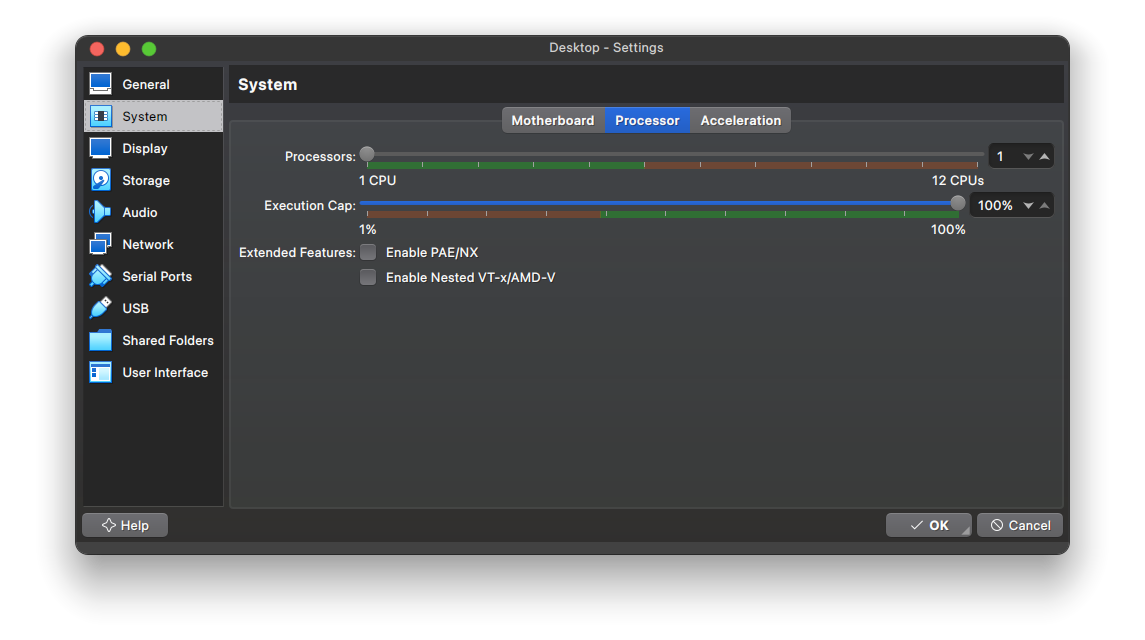
\includegraphics[width=\linewidth]{./imgs/Hinh-9.png}
  \caption{\bfseries Số Core CPU của Desktop}
  \label{fig:desktop-processor}
\end{minipage}



\begin{minipage}{.93\linewidth}
  \captionsetup{type=figure, skip=-15pt}
  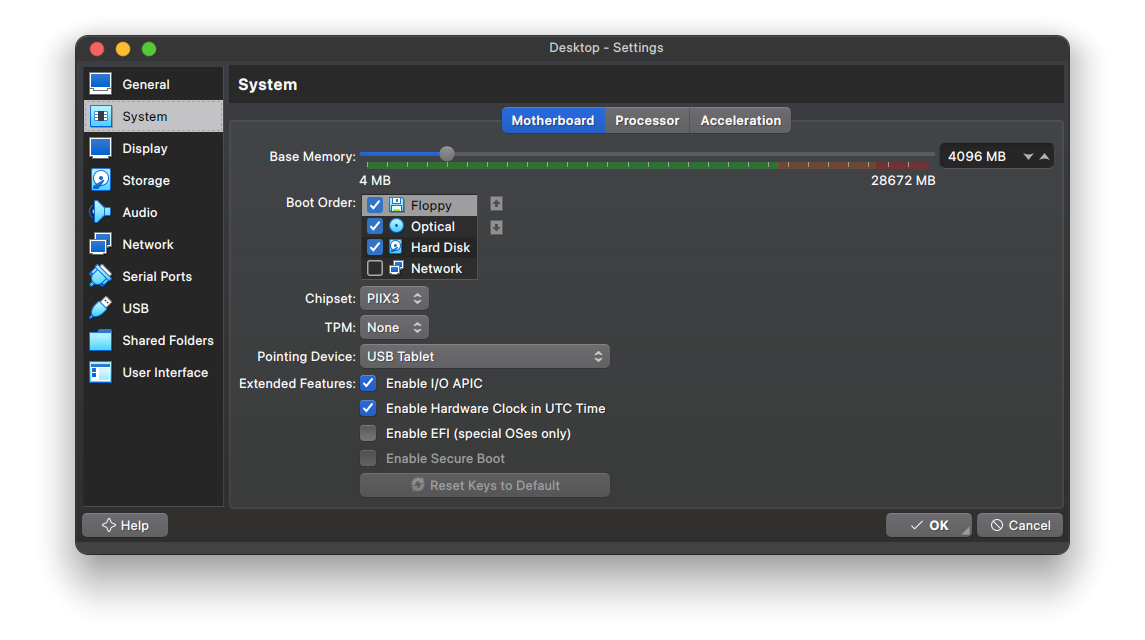
\includegraphics[width=\linewidth]{./imgs/Hinh-8.png}
  \caption{\bfseries Dung lượng Ram của Desktop}
  \label{fig:desktop-ram}
\end{minipage}


\begin{minipage}{.93\linewidth}
  \captionsetup{type=figure, skip=-15pt}
  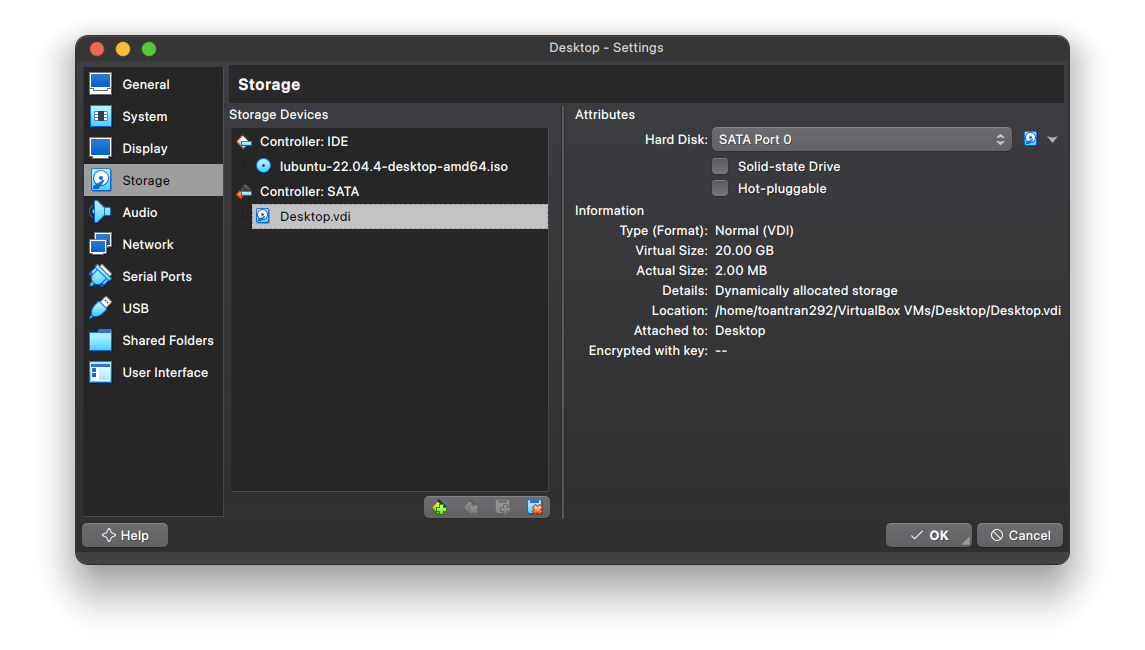
\includegraphics[width=\linewidth]{./imgs/Hinh-10.png}
  \caption{\bfseries Dung lượng ổ cứng của Desktop}
  \label{fig:desktop-disk}
\end{minipage}


\begin{minipage}{.93\linewidth}
  \captionsetup{type=figure, skip=-15pt}
  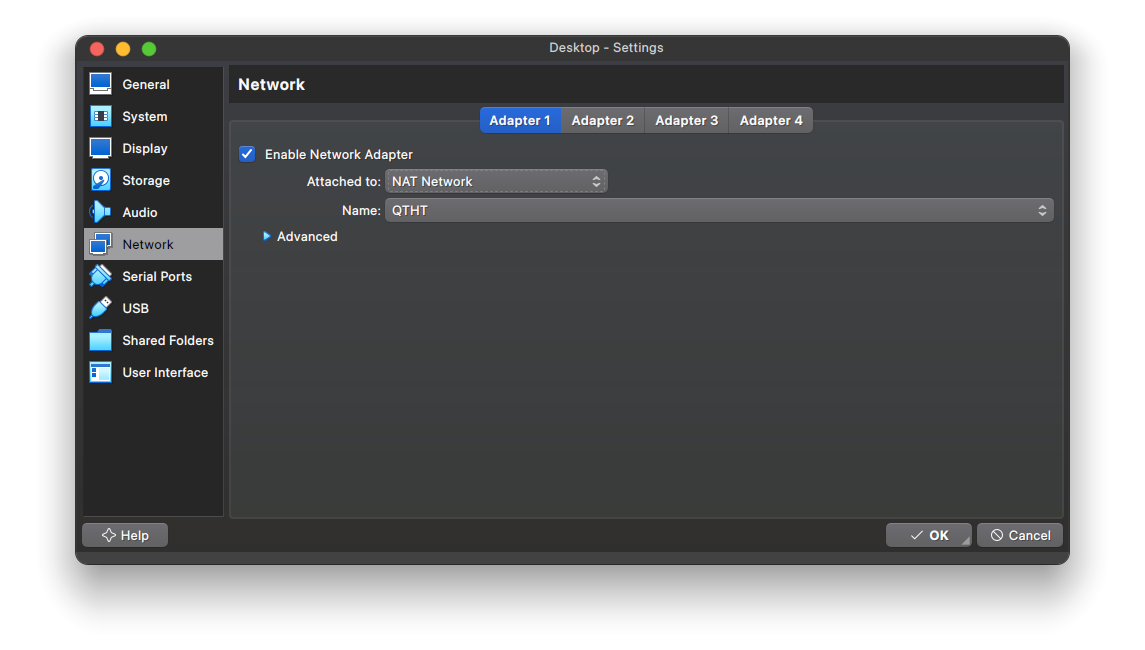
\includegraphics[width=\linewidth]{./imgs/Hinh-11.png}
  \caption{\bfseries Cấu hình mạng máy tính Desktop}
  \label{fig:desktop-network-1}
\end{minipage}

